\documentclass[article]{jss}
\usepackage{natbib}
\usepackage{amssymb}
\usepackage{amsmath}

%%%%%%%%%%%%%%%%%%%%%%%%%%%%%%
%% declarations for jss.cls %%%%%%%%%%%%%%%%%%%%%%%%%%%%%%%%%%%%%%%%%%
%%%%%%%%%%%%%%%%%%%%%%%%%%%%%%

%% almost as usual
\author{Clifford Anderson-Bergman\\Gladstone Institutes, UCSF}
\title{\pkg{icenReg}: Regression Models for Interval Censored Data in R}

%% for pretty printing and a nice hypersummary also set:
\Plaintitle{icenReg: Regression Models for Interval Censored Data in R} %% without formatting
%\Shorttitle{\pkg{foo}: A Capitalized Title} %% a short title (if necessary)

%% an abstract and keywords
\Abstract{
  Algorithms for fitting a semi-parametric Cox-PH model for interval censored data have existed in the literature for over 15 years at the time of this writing. However, currently there are no reliable \proglang{R} packages for fitting such models for the analysis of real data. The established algorithms are by no means trivial, so it is unreasonable to think that a researcher would rewrite these algorithms to analyze their own data set. To fill this gap, we created the \proglang{R}-package \pkg{icenReg} whose centerpiece is an algorithm for computing the semi-parametric Cox-PH  or proportional odds model based on a combination of established algorithms for the Cox-PH model and similar problems. Standard errors are estimated via bootstrapping, which is set up to take advantage of multiple cores with minimal effort by the user. In addition, we provide functions for fitting Cox-PH and proportional odds parametric models for interval censored data and functions for easy diagnosis of both parametric assumptions and covariate effects.  
}
\Keywords{interval censoring, Cox-PH, proportional odds, survival analysis, semi-parametric regression, multiple imputations}
%\Plainkeywords{keywords, comma-separated, not capitalized, Java} %% without formatting
%% at least one keyword must be supplied

%% publication information
%% NOTE: Typically, this can be left commented and will be filled out by the technical editor
%% \Volume{50}
%% \Issue{9}
%% \Month{June}
%% \Year{2012}
%% \Submitdate{2012-06-04}
%% \Acceptdate{2012-06-04}

%% The address of (at least) one author should be given
%% in the following format:
\Address{
  Clifford Anderson-Bergman\\
  Gladstone Institutes\\
  University of California, San Francisco\\
  1650 Owens Street\\
  San Francisco, CA\\
  E-mail: \email{cliff.andersonbergman@gladstone.ucsf.edu}\\
}
%% It is also possible to add a telephone and fax number
%% before the e-mail in the following format:
%% Telephone: +43/512/507-7103
%% Fax: +43/512/507-2851

%% for those who use Sweave please include the following line (with % symbols):
%% need no \usepackage{Sweave.sty}

%% end of declarations %%%%%%%%%%%%%%%%%%%%%%%%%%%%%%%%%%%%%%%%%%%%%%%


\begin{document}

%% include your article here, just as usual
%% Note that you should use the \pkg{}, \proglang{} and \code{} commands.

\section[intro]{Introduction}

	In the setting of survival analysis, interval censored data occurs when an event time is known only up to an interval. There are two common forms of interval censored data: case I, or current status data, occurs when each subject is observed at a single (random or fixed by design) time, and all that is recorded is whether the event of interest has occurred or not. This results in all subjects being either left or censored. A classic dataset includes mice that are sacrificed at random times and inspected for lung tumors (\cite{mice_tumors}). If tumors were detected, the mice were recorded to be left censored at time of sacrifice. If no tumors were found, they were recorded as right censored. Case II, or general interval censoring, can include left censored, right censored, uncensored and observations that are censored but neither right nor left censored. The last type of censoring can occur if a subject is regularly inspected and all that is known is that the event of interest occurred between inspections. A classic case II interval censored data set includes semi-regular dentist visits by children, with the event of interest being emergence of permanent teeth (\cite{toothStudy}). By selecting the last visit without permanent teeth and the first with permanent teeth, the researchers knew the event time up to an interval. 
	
	Standard parametric models can be used and are fairly straight forward to implement using standard algorithms. Implementations of general location-scale transformed models (the most well known being the accelerated failure time model) can be found in the \proglang{R}-package (\cite{R}) \pkg{survival} (\cite{R_surv}, \cite{R_surv_book}), fit with the \code{survreg} function. These models must be used with some caution: they are heavily influenced by the choice of parametric model, for which the model inspection can be extremely difficult due to the interval censoring. 
	
	Because of this, non-parametric models are often used, at least for diagnosistics. For univariate data, the non-parametric maximum likelihood estimator (NPMLE) is often preferred (\cite{Turnbull_1976}), which can be thought of as a generalization of the Kaplan Meier curves (\cite{KM_curve}) for interval censored data. This can be fit by the function \code{EMICM} in the package \pkg{Icens} (\cite{Icens}, \cite{EMICM}). Alternatively, this can fit by the function \code{computeMLE} in the package \pkg{MLEcens} (\cite{MLEcens}, \cite{SupRedAlg}) which, in the current implementations, is much faster. In terms of statistical properties NPMLE is notoriously inefficient; for case I interval censored data, the convergence rate has been shown to be $n^{1/3}$ (\cite{Case1Con}) instead of the more standard $n^{1/2}$, while for case II the convergence rate has been conjectured to be $n^{1/2} - n^{1/3}$ (\cite{Case2Con1}, \cite{Case2Con2}), depending on the severity of the interval censoring. 
	 
	 For non-parametric comparison of different stratum, a log-rank test can be used (\cite{ic_logrankTests}). However, this is complicated by the fact that the NPMLE is characterized by a large number of parameters, many of which many be on the boundary. Alternatively, permutation tests may be used to compare separate groups. \proglang{R} implementations of both these tests can be found in the \proglang{R}-package \pkg{interval} (\cite{intervalPackage}), called by the function \code{ictest}.  
	 
	For semi-parametric regression modeling of interval censored data, a Cox-PH model (\cite{CoxPH}) can be used (\cite{ic_coxph}). Unlike the case of right censored data, the regression parameters cannot be estimated without estimating baseline survival distribution. The model can still be kept semi-parametric by using the NPMLE as the baseline survival distribution. Interestingly, even though the rate of convergence can be as low as $n^{1/3}$ for survival estimates based on the NPMLE, it has been shown regression coefficients converge at the standard $n^{1/2}$ rate and are asymptotically normal (\cite{ic_coxph_asyp}), allowing for efficient comparisons with the semi-parametric Cox PH model. Inference on the regression parameters can be done using bootstrap standard errors (\cite{bootstrap}). Alternatively, a semi-parametric proportional odds model can be used (\cite{propOdds1}, \cite{propOdds2}). 

	It was shown that the model can be fit with an ICM algorithm (\cite{basicICM}, \cite{coxphICM}). This algorithm has been implemented in \proglang{R} in the package \pkg{intcox} (\cite{intcox}). However, there are several shortcomings in this package which make it inadequate for general data analysis: first and foremost, the algorithm does appear to be able handle uncensored observations in the data, implying it would not be able to handle general case II interval censoring. We are not sure what causes this problem. Similarly, the algorithm would often immediately fail in the case of discrete censoring, even if all the observation intervals have strictly positive interval lengths. Furthermore, no standard errors are provided for the estimates (although this can be overcome via bootstrapping). Finally, under the standard settings the algorithm prematurely converges quite often, leading to regression estimates that can be off by a significant amount. For example, in a recent general tutorial on interval censored data (\cite{ic_tutorial}), the authors use \code{intcox} on a sample dataset, which results in final log likelihood of -5368.38 and regression parameters 0.288 and 0.316. However, rerunning this analysis, we see that \code{intcox} reports an error after the first iteration. We found that at the MLE, the log likelihood was in fact -5138.57, with regression estimates of 0.322 and 0.337, using the software we provide. Given these issues, we would not consider \pkg{intcox} reliable for general analysis of real data in it's current form. 
	
	To the best of our knowledge, there is no \proglang{R}-package available for fitting a semi-parametric proportional odds model for interval censored data. 
	 
	 In \pkg{icenReg}, we provide tools intended for analysis of real data. In particular, we present a more reliable and considerably faster algorithm for fitting the semi-parametric Cox-PH and proportional odds models through the function \code{ic_sp}. The algorithm iterates between a conditional active set step to update the baseline parameters and a conditional Newton Rhapson algorithm to update the regression parameters. This more advanced algorithm allows for much faster and more reliable computation, allowing for quick bootstrapping for moderately sized ($n \leq 10,000$) datasets. We also provide routines for fully parametric Cox-PH and proportional odds regression models via \code{ic_par}. Finally, we provide functions \code{diag_baseline} and \code{diag_covar} for easy visual review of both parametric assumptions and covariate effects which relies on our semi-parametric models. 
	 
	 In section \ref{sec:alg1}, we describe our algorithm to fit the semi-parametric model and compare results to those found in \pkg{intcox}. 
	 
\section[alg1]{Description of algorithm for semi-parametric models}
\label{sec:alg1}
%\section{Likelihood Function for Semi-parametric Cox-PH Model}
	 
	 For characterization of the semi-parametric Cox-PH and proportional odds models, we start from the assumption of independence of the event time and censoring mechanism. We also use the standard interval notation that for subject $i$, $l_i$ and $r_i$ are the left and right side of their ``observation interval" (\emph{i.e.} the interval for which the event is known to have occurred). This allows for left censoring ($l_i = 0$), right censoring ($r_i = \infty$), uncensored observations ($l_i = r_i$) and general interval censoring. From here, we construct the Cox-PH likelihood function as
	 
	 \[
	 \displaystyle \sum_{i = 1}^n \log \left( S_o(l_i)^{e^{X_i \beta} } - S_o(r_{i+})^{e^{X_i \beta}} \right)
	 \]
	 
	 where $S_o$ is the baseline survival function, $X_i$ are an individual's covariates with no intercept and $\beta$ is a vector of coefficients. Similarly, we can define the likelihood function in the proportional odds model as
	 
	  \[
	 \displaystyle \sum_{i = 1}^n \log \left( \frac{S_o(l_i) e^{X_i \beta}}{S_o(l_i) e^{X_i \beta} -S_o(l_i) + 1 } -\frac{S_o(r_i) e^{X_i \beta}}{S_o(r_i) e^{X_i \beta} -S_o(r_i) + 1 }  \right)
	 \]
	 
	 It is worth noting that while for continuous distributions, censored and uncensored observations must be handled differently (\emph{i.e.} with the survival distribution and probability density function respectively), in the case of the semi-parametric estimator, it has been shown that the baseline distribution can treated as a discrete distribution and so $S_o(t) - S_o(t_+) > 0$ if probability mass is placed at $t$. In fact, it has been shown that the MLE places positive probability only inside \emph{Turnbull intervals} (\cite{Turnbull_1976}), $\emph{i.e.}$ intervals such that the left side of the interval is the left side of an observation interval, the right side of the interval is the right side of (possibly a different) observation interval, with no ends of any other intervals in between.   Uncensored observations are considered to be intervals of length 0, and so automatically become Turnbull intervals. With this in mind, the above likelihood functions can be written as a function of a finite number of parameters by replacing $	S_o(x_i)  $
with  
\[
1 - \displaystyle \sum_{T_j < x_i} p_j 
\]
\[
\text{ such that }   p_j \geq 0, \sum p_j = 1
\]	 
%	 \[
%	 \displaystyle \sum_{i = 1}^n \log \left[  
%	 	\left(1 - \sum_{T_j < l_i} p_j \right) ^ {exp(X_i \beta)} - \left(1 - \sum_{T_j \leq r_i} p_j \right) ^{exp(X_i \beta)}
%	 \right]
%	 \] 
	 where $p_j$ is the probability mass assigned to Turnbull interval $T_j$. This is a slight abuse of notation, as comparing an interval ($T_j$) to a point ($l_i$ or $r_i$) is typically ill defined. In our case, by definition of the Turnbull intervals, if $l_i$ or $r_i$ (\emph{i.e.} the ends of an observation interval) are greater than or equal to any single point in a Turnbull interval, they are greater than or equal to all points in the Turnbull interval. Likewise for less than or equal to. Under this parameterization, we can characterize the MLE with a finite number of parameters; the regression parameters $\beta$ and baseline distribution probability masses $p$. 

	To add in computation, we optimize the likelihood on the cumulative hazard scale rather probability masses. Reparameterizing the discrete survival function as a cumulative hazard function, we can describe the baseline cumulative hazard as	
	\[
	\Lambda(x_i, H) = 	\begin{cases} -\infty 	& \text{if } x_i < T_1\\
							      H_j	& \text{if } x_i \geq T_j \cap x_i < T_{j+1}	\\
							      \infty 	& \text{if } x_i > T_k	
					\end{cases}					
	\]
	\[
	\text{such that }H_j \leq H_{j+1}
	\]
	where $k$ is the number of Turnbull intervals.
	
	We also define the function which links the baseline cumulative hazard to the survival function conditional on the covariates as $f_m(h | X, \beta)$, where $m$ represents the model selected. For the Cox-PH model, we have
	
	\[
	f_{ph}(h |X, \beta) = e^{-e^{h + X \beta } }
	\]
	
	For the proportional odds model, we have 
	
	\[
	f_{po}(h | X, \beta) = \frac{ e^{ -e^h + X \beta} } { e^{ -e^h + X \beta}  - e^{-e^h} + 1  }
	\]
	
	Using this, our algorithm maximizes the following function:
	
	\[
	\displaystyle \sum_{i = 1}^n \log \left(  f_m( \Lambda(l_i, H) | X_i, \beta)  - f_m( \Lambda(r_i, H) | X_i, \beta)		\right)
	\]
	\[
	\text{ such that } H_j \leq H_{j+1}
	\]
	
	Each iteration of our algorithm included a conditional Newton-Raphson step which updates the regression parameters and an active set step which updated the baseline hazard function. In active set step, a pool-adjacent violators algorithm is used to optimize the baseline hazard function while still respecting the monotonic constraint of the cumulative hazard. 
	
	\begin{table}
	\begin{center}
	\begin{tabular}{| c | c | c |}
	
		\hline
				\multicolumn{3}{| c |}{Proportional Hazards} \\
		\hline
						& Mean Time 			&  Mean $\hat{lk} - lk$\\
	\hline
	\multicolumn{3}{| c |}{$ n = 100$}	\\
	\hline
	
	\code{ic_sp}			&	0.006			&		0.000					\\
	
	\code{intcox}: default		&	0.155			&		0.253				\\
	
	\code{intcox}: strict		&	1.142			&		0.010					\\
	
	\hline
	\multicolumn{3}{| c |}{$ n = 500$}	\\
	\hline
	
	\code{ic_sp}			&	0.032			&		0.000				\\
	
	\code{intcox}: default		&	0.351			&		1.797			\\
	
	\code{intcox}: strict		&	2.754			&		0.078			\\


	\hline
	\multicolumn{3}{| c |}{$ n = 1,000$}	\\
	\hline
	
	\code{ic_sp}			&		0.082		&		0.000					\\
	
	\code{intcox}: default		&		0.744		&		5.753				\\
	
	\code{intcox}: strict		&		6.036		&		0.165				\\
	
	\hline

	\multicolumn{3}{| c |}{$ n = 5,000$}	\\
	\hline
	
	\code{ic_sp}			&		0.787		&		0.000				\\
	
	\code{intcox}: default		&		4.258		&		87.65			\\
	
	\code{intcox}: strict		&		86.06		&		0.953			\\
	
	\hline

	\end{tabular}
	\caption[Average computation times]{Average computation times in seconds and average difference in final log likelihood from MLE. \code{intcox}: default refers to default settings of the \code{intcox} function, while \code{intcox}: strict refers to the same function but with a stricter convergence criteria.}	
	\label{table:speedTable}
	\end{center}
	\end{table}
	
	
	\begin{table}
	\begin{center}
	\begin{tabular}{| c | c |}
	
		\hline
		\multicolumn{2}{| c |}{Proportional Odds}\\
		\hline
		$n = 100$		&			0.005			\\
		\hline

		\hline
		$n = 500$		&			0.018			\\
		\hline 
		
		\hline
		$n = 1000$		&			0.034		\\
		\hline
		
		\hline
		$n = 5000$		&			0.198		\\
		\hline
	\end{tabular}
		\caption[Average computation times2]{Average computation times in seconds for the \code{ic\_sp} function with proportional odds model. Data simulated by \code{simIC\_weib}. }

	\label{table:speedTable2}
	\end{center}
	\end{table}
	
	% However, even with this issue, there is little question that \code{ic_ph} outperforms \code{intcox}.
		
	To examine the speed of the algorithms, we simulated interval censored data (via the function \code{simIC_weib}) with two covariates and sample sizes $n$ = 100, 500, 1,000 and 5,000, where the true baseline distribution was weibull(2,2). For the censoring mechanism, we used a case II interval censoring mechanism in which two inspections were used, with inspection time simulated according to a uniform(0, 2.5) distrbution. 

	Fair comparison of the speed of our algorithm with that found in \pkg{intcox} is somewhat confounded by the fact that the algorithm called by \code{intcox} typically prematurely terminates, biasing the speed estimates. Even still, it is quite clear that our algorithm is both much faster and more reliable. For a complete comparison, we used both the default settings and also supplied a more strict convergence criteria to \code{intcox}. With each dataset, we fit \code{ic_sp}, \code{intcox} with default settings and \code{intcox} with stricter convergence criteria (referred to as \code{intcox}:default and \code{intcox}:strict respectively). For the \code{intcox}:strict, we set the argument \code{epsilon} = $10^{-6}$ (this is refers to the required difference in likelihood between iterations for termination. Default is $10^{-4}$). For each sample size and algorithm configuration, we recorded mean time to algorithm termination and mean difference of final likelihood for each configuration compared with the maximum likelihood of all three configurations. At each configuration, 100 simulated datasets were fit. The algorithm used in \code{intcox} very frequently failed with discrete censoring, reporting algorithm failure in the first iteration over half the time. Because of this, the speed of the \code{intcox} algorithm was not examined for discrete censoring.  Results are presented on table \ref{table:speedTable}.  We found \code{ic_sp} significantly outperformed the other configurations in all situations. It appeared that the competitive speed advantage of \code{ic_sp} technically decreased as $n$ increased (in fact, with $n = 5,000$, \code{intcox}:default stops much faster \code{ic_sp}), but this seems to be a result of the stopping criteria of \code{intcox} being too lax and preforming worse as $n$ increases: even for \code{intcox}:strict, at $n = 5,000$, the average difference in final log likelihood implies that the results should not be trusted. 
	
	We also clocked the algorithm for proportional odds under similar scenarios, but simulated proportional odds event times rather than proportional hazards. There is no existing algorithm that we are aware of to clock against. Results are shown on table \ref{table:speedTable2}.
	
	All simulations were run on a 2014 Macbook Pro with a 2.2 GHz i7 processor. 
	
	
	%In the continuous censoring with $n = 5,000$, the relatively speed advantage of \code{ic_ph} seemed was technically heavily reduced; in fact, the standard settings for \code{intcox} was much faster to terminate. However, this seems to be a result of very premature termination of the algorithm rather than computational advantage, as \code{intcox}:default was found to be extremely far from the MLE, while \code{intcox}:strict was several fold slower and still fairly far from the MLE on average. In every single dataset fit, the likelihood of the \code{ic_ph} was higher than for \code{intcox}.
	
	
\section[par]{Algorithm for Parametric Models}	
\label{sec:alg_par}	

	When parametric models are considered, the likelihood function must treat uncensored observations in a distinct manner. In the case of the Cox-PH model, the likelihood can be written as
	
	\[
		\displaystyle \sum_{i = 1}^{n_1}  \log \left( e^{X_i \beta }f_o(t_i | \alpha)	 S(t_i | \alpha) ^ {e^{X_i \beta- 1}} \right) +
		\displaystyle \sum_{i = n_1 + 1}^{n_1 + n_2}  \log \left( S_o(l_i | \alpha)^{e^{X_i \beta} } - S_o(r_{i+} | \alpha)^{e^{X_i \beta}} \right)
	\]

where $\alpha$ are the parameters associated with the baseline distribution, $\beta$ are the regression parameters, $X_i$ are an individual's covariates, $f_o$ and $S_o$ are the baseline density and survival functions, with the first $n_1$ subjects being the uncensored subjects, and the remaining $n_2$ subjects are censored. 

For the proportional hazards model, the likelihood function can be written as 

\[
	\displaystyle \sum_{i = 1}^{n_1}	 \log \left( \frac{f_o(t_i | \alpha) e^{X_i \beta}} {( S_o(t_i | \alpha) e^{X_i \beta} - S_o(t_i | \alpha)  + 1)^2}	\right)
\]
\[
	+ \displaystyle \sum_{i = n_1 + 1}^{n_1+n_2} \log \left( \frac{S_o(l_i | \alpha) e^{X_i \beta}}{S_o(l_i | \alpha) e^{X_i \beta} -S_o(l_i | \alpha) + 1 } -\frac{S_o(r_i | \alpha) e^{X_i \beta}}{S_o(r_i | \alpha) e^{X_i \beta} -S_o(r_i | \alpha) + 1 }  \right)
\]

	In all the parametric families we consider, the parameter space $\alpha$ is transformed such that it is defined on $\mathbb{R}^k$, where $k$ is the number of parameters of the parametric family. For example, the exponential family, log rate is used instead of rate. 

	To maximize this likelihood function, a two step algorithm is used. A simple conditional Newton-Raphson step is used to update the regression parameters, as the function will be concave under mild conditions. The log likelihood function is not necessarily concave as a function of the baseline parameters, and it was occasionally found to be non-locally concave for poor starting choices of $\alpha$. To handle this, the algorithm would first check if the Hessian was negative definite. If so, a conditional Newton-Raphson step was used. If not, a conjugate gradient step was used. 
	
	To compare this algorithm with an established implementation, we simulated 100 datasets with our function \code{simIC_weib} with $n = 100,000$ and fit the data with both our algorithm with a Cox-PH weibull model and \pkg{survival}'s \code{survreg} function. Although \code{survreg} fits a weibull aft model by default, this leads to the same maximum likelihood, as for the weibull distribution, the aft and Cox-PH models are identical up to a linear transformation of variables. Slight modification of the simulated data was required as \code{survreg} does not allow for the left side of intervals to be 0 or the right side to be $\infty$. The two implementations reliably found the same estimate;  the maximum absolute difference in final log likelihood observed was  $3.5 \times 10^{-9}$. It was found that \code{survreg} was slightly faster, with an average computation time of 0.79 seconds vs 3.88 seconds. Currently, our algorithm uses numeric derivatives and we believe that replacing them with analytically calculated derivatives could lead to similar speed as \code{survreg}. 

{\section[diagnosis] {Diagnostic Tools} }	

	When fitting parametric regression models, the researcher makes an assumption about the effect of the covariates and the baseline parametric model. When fitting a semi-parametric model, the second assumption is dropped. Either way, it is important to assess the validity of the assumptions. With interval censored data, this can be fairly difficult. Our package includes easy to use routines for examining both sets of assumptions, both of which use the semi-parametric model. 
	
	To examine the parametric baseline assumption, \code{diag_baseline} fits and plots the baseline survival distribution of a variety of parametric choices. It also plots the semi-parametric estimated baseline distribution. This can help an investigator assess if there appears to be a systematic deviation from the assumed baseline distribution. 
	
	To examine the functional form of the covariates, we take use the fact that for both models, there is a transformation of the survival function such that differences in covariate effects will result in constant differences. For the proportional hazards model, note that
	
\[
\log(-\log( S(t | X, \beta) ) ) = \log ( -\log( S_o( t ) ^{e^{X \beta} } ) ) =X \beta + \log( - \log( S_o( t) ) ) 
\]

Likewise, for the proportional hazards model, note that 

\[
\log \left( \frac{S(t | X, \beta) } { 1 - S(t | X, \beta) } \right) = \log \left(	\frac{\left(\frac{S_o(t) e^{X \beta} } {S_o(t) e^{X \beta} - S_o(t) + 1}	\right)}{\left (\frac{S_o(t) e^{X \beta} } {S_o(t) e^{X \beta} - S_o(t) + 1}	\right)-1}	\right) = 
\]

\[
\log \left(	\frac{\left(\frac{S_o(t) e^{X \beta} } {S_o(t) e^{X \beta} - S_o(t) + 1}	\right)}{\left (\frac{ S_o(t) - 1 } {S_o(t) e^{X \beta} - S_o(t) + 1}	\right)}	\right) 
= X \beta \log \left(\frac{ S_o(t) } { S_o(t) - 1 } \right)
\]

	To investigate whether the functional form is appropriate for a given covariate, \code{diag_covar} first stratifies the dataset on different levels of that covariate. It then fits a semi-parametric model for each strata and plots the given transformation of the baseline survival functions. If functional form of the covariate is correct, the difference between the two strata's transformed baseline should be approximately constant. To help visualize the difference, the average of all the strata is subtracted off of each strata by default. 

{\section[use]{Using \pkg{icenReg}}	
	
	The core functions in \pkg{icenReg} are \code{ic_sp} and \code{ic_par} for fitting the semi- and fully-parametric Cox-PH models respectively. Results of the fitted models can be viewed with the standard \code{summary} method. Plots of estimated survival curves can be viewed via the \code{plot} method. 
	
	Alternatively, the estimated survival curves can be extracted by the \code{getSCurves} function. For the sake of demonstration, \pkg{icenReg} includes the function \code{simICPH_beta}, which simulates proportional hazards data with a beta baseline distribution and \code{mdata}, a real current status data set from \cite{mice_tumors}.
	
	The functions \code{ic_ph} and \code{impute_ic_ph} shares many arguments. In particular, they both include the standard arguments \code{formula} and \code{data}. In the \code{formula} argument, the response must be a \code{Surv} object with \code{type = "interval2"}. These functions also include the arguments \code{useMCores = F}, a logical indicator for whether multiple cores should be used for the imputation or bootstrap step and \code{seed = NULL}, a numeric value for which seed will be passed to \code{set.seed} before the bootstrap or imputation samples are taken. If \code{seed = NULL}, a random seed is generated and passed to \code{set.seed}. The arguments \code{bs_samples = 20} and \code{imps = 100} refer to the number of bootstrap or imputation samples to be taken. The default values are lower than recommended for inference; this is so users can estimate the time needed to run the necessary samples. Unique to \code{impute_ic_ph} are the arguments \code{eta = 1e-10} and \code{rightCenVal = 10000}. This is because the \pkg{survival} function \code{survreg} used for the imputation model cannot handle values of 0 or \code{Inf}, so values less than \code{eta} are replaced with \code{eta} and values greater than \code{rightCenVal} are replaced with \code{rightCenVal}. In some cases, it may be necessary to supply a larger value of \code{rightCenVal}. 
	
	The \code{summary} function is used in the standard manner. For the \code{plot} function for \code{ic_ph} fits, if only the fit is provided, the baseline survival distribution will be plotted. Alternatively, the second argument supplied to \code{plot} can be a new data.frame, with matching variables names to those found in the original dataset. In this case, \code{plot} will plot the survival curve for each set of covariates. A legend will be plotted using the rownames of the data.frame. For custom plots, the function \code{getSCurves} can be used to extract the survival curves, with similar arguments to \code{plot} (\emph{i.e.} first argument is the fit, optional second argument can be a new data.frame). 
	
	For demonstrative purposes, the package includes a function \code{simICPH_beta}, which simulates data from a Cox-PH model with a beta baseline distribution. The arguments accepted are \code{n}, the number of subjects simulated, \code{b1} and \code{b2}, the coefficients for the covariates, \code{inspections = 1}, the number of inspection times (default is one inspection, resulting in current status data), \code{shape1} and \code{shape2}, the parameters of the baseline distribution and \code{rndDigits}, the number of digits that the inspection times will be round to (\code{rndDigits = NULL} implies no rounding). The covariates associated with \code{b1} and \code{b2} are distributed \code{rnorm(n)} and \code{rbinom(n, 1, 0.5) - 0.5} respectively. The reason a beta distribution was chosen is that this will lead to the imputation model assuming a very inappropriate baseline distribution (Weibull) and one can see that if the number of \code{inspections} is low, the imputation model will lead to heavy bias. However, if the number of \code{inspections} is high, we will see the bias is fairly small. We leave implementation of this to the curious reader. 
	
	In order to use parallel computation of either bootstrap or imputation samples, we take advantage of the \pkg{foreach} package (\cite{foreach}). The user must make and register a cluster via \pkg{doParallel}'s \code{makeCluster} and \code{registerDoParallel} (\cite{doParallel}). We demonstrate this in the next section. 
	
{\section{Example Analysis}}
	 For our example, we will use the dataset \code{mdata} provided in our package. This dataset borrows from \cite{mice_tumors}. In this study, RFM mice were sacrificed and examined for lung tumors. If tumors were found, the mouse was considered left censored with the inspection time being equal to age at sacrifice. If no tumors were found, the mouse was considered right censored. Mice were placed in two different environments: conventional environments and germ free environments. In the \code{mdata} dataset, \code{l} represents the left side of the observation interval, \code{u} represents the right side and \code{grp} is a factor representing the environment the mouse was placed in. 

	Below we analyze the data using both \code{ic_ph} and \code{impute_ic_ph}. To begin with, we will use the package \pkg{doParallel} to set up a cluster.

\begin{CodeChunk}
\begin{Code}
> library(doParallel)
> myCluster <- makeCluster(3, type = 'FORK')
> registerDoParallel(myCluster)
\end{Code}
\end{CodeChunk}	
	
	Next, we will load the data and fit the two models.
	
\begin{CodeChunk}
\begin{Code}
data(mdata)
sp_fit <- ic_ph(Surv(l, u, type = 'interval2') ~ grp, 
	data = mdata, bs_samples = 500, useMCores = T)
mi_fit <- impute_ic_ph(Surv(l, u, type = 'interval2') ~ grp, 
	data = mdata, imps = 500, useMCores = T)
\end{Code}
\end{CodeChunk}
	
	We viewed the results of the two fits with the \code{summary} function. 

\begin{CodeChunk}
\begin{Code}
> summary(sp_fit)

Semi Parameteric Cox PH model for interval censored data
Call = 
ic_ph(formula = Surv(l, u, type = "interval2") ~ grp, data = mdata, 
    bs_samples = 500)

    Estimate Exp(Est) Std. Error z-value      p
grp   0.6277    1.873     0.4087   1.536 0.1246

final llk =  -76.53436 
Iterations =  26 
Bootstrap samples =  500 
> summary(mi_fit)

Multiple Imputations Cox PH model for interval censored data
Call = 
impute_ic_ph(formula = Surv(l, u, type = "interval2") ~ grp, 
    data = mdata, imps = 500)

      Estimate Exp(Est) Std. Error z-value       p
grpge   0.7409    2.098     0.3135   2.363 0.01811

number of imputations =  500 
\end{Code}
\end{CodeChunk}

	For visualization, we plot the \code{ic_ph} fit for the two groups. 
	
\begin{CodeChunk}
\begin{Code}
> newdata <- data.frame(grp = c('ce', 'ge'))
> rownames(newdata) = c('Conventional Environment', 'Germ Free Environment')
> plot(sp_fit, newdata)
> sCurves <- getSCurves(sp_fit, newdata)
\end{Code}
\end{CodeChunk}

	We note that the imputation model results in slightly different estimates than the semi-parametric model, and slightly higher standard errors. This is due to the relative wide observational intervals, leading to heavy influence from the imputation model. 
	
	Based on our findings, we would conclude that while it was estimated that mice in the germ free environment were at higher risk to develop tumors than those in the conventional environment, we did not find enough evidence to reject the notation that the hazard rates might be equal. This implies we trusted the results of the semi-parametric model over the parametric imputation model. We decided on this because the observation intervals were relatively wide, and so the parametric imputation model could result in heavy biases. 

\begin{center}
{\begin{figure}
\centering
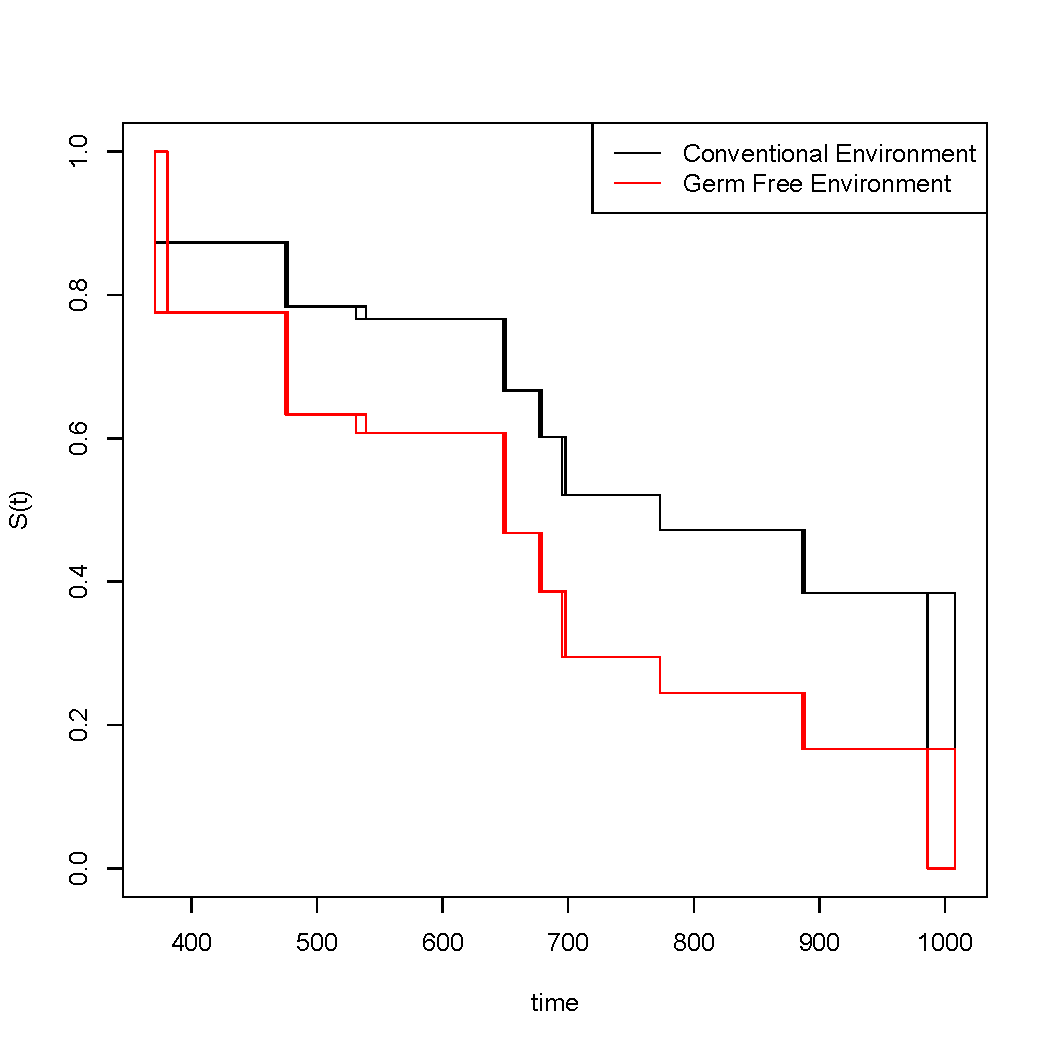
\includegraphics{mousePlot.pdf}
\caption{Plotted survival curves for \code{mdata} dataset}
\label{plot:tooth}
\end{figure}}
\end{center}	

%{\section[inspect]{Examination of Estimator Characteristics}
%\label{sec:inspect}}

%	Using our new software, we present a very brief investigation of the operating characteristics of our estimators. We address two topics: first, we re-investigate the issues of upward bias of regression coefficients for the semi-parametric model found in Wei Pan 1999. Second, we investigate the sensitivity of the parametric assumption of the multiple imputations model. In both cases, we 	
	
	
{\section[future]{Future Expansions}} 

	We have several plans to expand \pkg{icenReg} to allow for easier analysis of interval censored data. In particular, we would like to provide user-friendly tools for model assessment, such as single function for stratifying the data on different levels of a covariate to examine the proportional hazards assumption. We are also interested in adding a semi-parametric proportional odds model, which should be able to use a similar algorithm as the proportional hazards model. 

%\bibliographystyle{te}	
\bibliography{icenReg}
	
	
\end{document}
